\section{Introduction}
\label{sec:caimanintro}

Accelerators have become of great interest to the computing community in the last few years~\cite{acceleratorsurvey}~\cite{nnacceleration}.  For specific applications or computations, specialized accelerators can provide significant performance improvements.  Using an accelerator, however, can require significant engineering effort and programmer expertise.

A major reason for the complexity of accelerator programming comes from the significant performance concerns that often appear when designing accelerator code.  Intuitively, when an engineer finds that an accelerator is needed for some task, performance is likely a consideration.  Since accelerators are often multithreaded, with specific requirements on data layouts or algorithm design.  These constraints and performance needs have led to years of research and industrial work to optimize accelerator \emph{kernels} (accelerator--only units of computation).  However, there is a significant cost in the communication between devices, and this  cost can be specifically painful when communication occurs as blocking the logic of a program.

This cost has been explored in several works in the form of automatic compiler optimizations~\cite{gpgpuopti} and code generation~\cite{cudaevolve}, which rely on either a compiler or learning model to generate communications or kernels based on some heuristic.  Despite these advances, anecdotally programmers are still optimizing performance--critical communication by hand.  This is (at least partially) due to the need for experimentation and profiling in performance--critical code, where a given solution may not perform optimally in all heterogeneous arrangements and even within a given codebase.

We argue, without any meaningful way to prove or refute this claim, that heterogeneous programming is diverse enough and performance--critical enough, that such hand--optimized solutions will continue to be important for kernel and shader engineers.  As a result, we propose a solution that raises the level of abstraction for performance engineering, but engineered so that the layer of abstraction being constructed is both transparent and decomposable.  We start by making more concrete the specific challenges we have observed while hand--optimizing kernels, specifically separating performance and correctness, and managing a combinatorial explosion of kernel interactions.

\subsection{Performance Experimentation}
\label{subsec:separation}

Our running example throughout this paper will be used to illustrate the performance trade--offs inherent in conditional logic and device synchronization.  Specifically, we will be building the \code{select_sum} function, which takes in three arrays `v1`, `v2`, and `v3`, and returns the sum of either `v2` or `v3` depending on the sign of `v1`.

A naive \texttt{Rust} solution for this might look something like the following (for some fixed size of array):
%
\begin{lstlisting}

select_sum(v1 : [i32; N1], v2 : [i32; N2], v3 : [i32; N3]) -> i32 {
  if sum(v1) < 0 {
    sum(v2)
  }
  else {
    sum(v3)
  }
}
\end{lstlisting}
%
Note that, in Rust, an expression without a \code{;} is equivalent to adding a \code{return}, so this code can be read as either returning the sum of \code{v2} or \code{v3}.

We might find that, for large arrays, this code is insufficiently performant in our setting. We might hope to be able to take an approach of the following Rust-like psuedocode, where we simply move our expensive \code{sum} operations onto the GPU:
%
\begin{lstlisting}
select_sum_2(v1 : [i32; N1], v2 : [i32; N2], v3 : [i32; N3]) -> i32 {
  if (sum_gpu(v1) < 0) {
    sum_gpu(v2)
  }
  else {
    sum_gpu(v3)
  }
}
\end{lstlisting}
%
Upon measuring the performance of this solution, however, we may find that this code isn't ``fast enough", even if we are using a highly--optimized GPU implementation of \code{sum}.  If we want to improve the performance of this code further, we have several options.  We could move this entire code onto the GPU (noting, crucially, that the GPU tends to perform poorly with conditions), but another reasonable approach would be to calculate each \code{sum} in advance, to avoid bottlenecking the next GPU calculation behind the CPU condition.  Concretely, in psuedocode, this implementation may look something like:
%
\begin{lstlisting}
select_sum_3(v1 : [i32; N1], v2 : [i32; N2], v3 : [i32; N3]) -> i32 {
  sum1 = sum_gpu(v1);
  sum2 = sum_gpu(v2);
  sum3 = sum_gpu(v3);
  if (sum1 < 0) {
    sum2
  }
  else {
    sum3
  }
}
\end{lstlisting}
%
To complicate this function even more, however, we may have a case where \code{v1} is a smaller array than \code{v2} or \code{v3}, and so sending \code{v1} to the GPU is introducing unnecessary overhead in our computation.  For this special case, we may need to consider the following function variation (even within our same program):
%
\begin{lstlisting}
// For N1 << N2,N3
select_sum_4(v1 : [i32; N1], v2 : [i32; N2], v3 : [i32; N3]) -> i32 {
  if (sum(v1) < 0) {
    sum_gpu(v2)
  }
  else {
    sum_gpu(v3)
  }
}
\end{lstlisting}
%
Note that, in this variation, we may find it optimal to revert to the original idea of having \code{sum_gpu} inside of the condition rather than before, since we are no longer blocking on communication between devices.

It is important to note that every one of these steps we described may depend on measuring performance in a specific setting, with specific array sizes, and even within specific functions.  The particular functions we wrote may or may not be optimal -- an analysis of our timing each variation of this function can be found in~\ref{sec:results} (including blindly moving the entire \code{select_sum} function to the GPU), but we can only show these results for a particular setting.  The takeaway, then, should be that a programmer may need to try each of these variations to find a performant solution, and may need to maintain multiple such functions (such as both \code{select_sum_3} and \code{select_sum_4}) in the same program, despite these functions doing the same computation!

To make matters worse, we are ignoring even more decisions that can be made between these black--box calls to \code{sum_gpu}.  The decision space here will be expanded on in~\ref{subsec:submission}, which will also expand on why these functions may be much harder to write than what we have shown here.  Before we continue, however, we need to explore another problem that arises from maintaining multiple definitions of \code{select_sum}.

\subsection{Combinatoric Explosion}
\label{subsec:combinatoric}

We have shown how to end up with several implementations of \code{select_sum}, where optimal performance may depend on setting-specific experimentation.  Another key aspect to optimizing heterogeneous performance, however, is optimizing for the context of surrounding functions.  This is suggested by our reliance on the condition \code{N1 << N2,N3}, which implies that we ought to be careful about which ``version" of \code{select_sum} to call based on information about the function calling \code{select_sum}.  We can extend this logic the other direction, and find cases where we may prefer one implementation of \code{sum_gpu} over another for a particular choice of \code{select_sum}, which we can name \code{sum_gpu2}.

Concretely, let us define some \code{complicated_function}, where we have three calls (at various points) to \code{select_sum}.  In--code, we can summarize this assumption as follows:
%
\begin{lstlisting}
fn complicated_function(...) {
  select_sum(...);
  // ...
  select_sum(...);
  // ...
  select_sum(...);
}
\end{lstlisting}
%
We may find, however, that \code{complicated_function} is optimized for a particular arrangement of \code{select_sum} implementations; for instance, we might experiment with the following arrangement:
%
\begin{lstlisting}
fn complicated_function(...) {
  select_sum_1(...);
  // ...
  select_sum_3(...);
  // ...
  select_sum_4(...);
}
\end{lstlisting}
%
This sort of experimentation can lead to an explosion of variations to try, where we may find that a given implementation of \code{sum_gpu} is preferable in a particular implementation of \code{select_sum} within this particular \code{complicated_function}, necessitating writing yet another variation of \code{select_sum}, which may require adjusting our other decisions, and so on and so forth.  In this manner, we can quickly end up writing an exponential number of variations of functions, or, practically, write a complex system of macros, comments, and/or implicit dependencies between code variants, with little in the way to help manage this design overhead.

\subsection{Caiman Languages}

To help address these problems with performance experimentation in heterogeneous programming, we introduce the Caiman language.  The core goal of Caiman is to provide a separation between the definition and the implementation of a function, and to allow these function implementations to be used interchangeably in implementation (with some important type--level protections).  In doing so, we make the following contributions in this work:
\begin{itemize}
\item We provide formal guarantees on multiple implementations for the same function \emph{specification}
\item We describe functions that are decomposable, in that a function implementation can be broken apart so that parts can be used by other implementations without duplicating the entire function, all without breaking Caiman's type--level guarantees of matching implementation to definition.
\item We describe and implement a system within Caiman to harness type--directed program synthesis to help reduce the overhead of performance experimentation and to allow transparency into compiler optimizations.
\item We provide a syntax and implementation for both human--writeable Caiman with the above guarantees, and a more precise Caiman IR for analysis and precise operational control.
\item We demonstrate the performance tradeoffs for several synthetic WebGPU kernels, and show that a Caiman implementation of these kernels allows a similar performance exploration.
\end{itemize}

\section{Related Work}

\paragraph{Scheduling Languages}

The philosophy of Caiman has overlap with scheduling languages such as Halide~\cite{halide}, Taco~\cite{taco}, and Exo~\cite{exo}.  The Caiman strategy of separating performance and implementation concerns is inspired by these sorts of scheduling languages, and indeed the direction for Caiman was initially written to be a scheduling language for heterogeneous interactions.  

Despite this core inspiration, Caiman navigates the specific challenges of heterogeneous programming differently than the scheduling languages we are aware of.   Most notably, Caiman emphasizes design for the combinatoric explosion of kernel design described in~\ref{subsec:combinatoric} and introduces type requirements for the multi--threading and condition logic present in heterogeneous decision making.

\paragraph{Heterogeneous Languages}

There have been a variety of heterogeneous programming languages in the last few years.  We highlight three well--known languages/APIs for comparison, but acknowledge there are many more projects that we will not specifically address.

CUDA~\cite{cuda} is a computational language for the GPU that allows for compiling C++ code with a GPU program while providing and API ``to use C++ as a high--level--language"~\cite{cudaguide}.  A key feature of this approach, however, is to make the interface between CPU and GPU very thin (CUDA code strongly resembles a C++ function).  This design makes writing code fairly straightforward, but can make extracting lower--level details for performance difficult.

OpenCL~\cite{opencl} is a widely used heterogeneous language solution, providing a language and API for a variety of heterogeneous settings.  OpenCL provides a similar toolset to CUDA, but is designed to be more general--purpose and more controllable than GPU compute, at the expense of being somewhat difficult to program and require domain--specific expertise.  SYCL~\cite{sycl} is an API built on top of (but separate to) OpenCL, and is meant to provide some of the higher--level benefits that can be seen with CUDA.

Vulkan~\cite{vulkan} is a graphics--specific API for the GPU that is meant to give more control over exact GPU implementation and communication details.  As with OpenCL, however, Vulkan can be difficult to use at scale due to the amount of domain--specific knowledge and optimization work needed.  Despite this, the recent interest in Vulkan gives an indication of the value that exposing detailed interfaces can have for developing performant systems.

Caiman is designed as an alternative approach to these heterogeneous APIs, with an emphasis on transparency in the boundary between abstractions and performance--critical implementation details.  A Caiman implementation could be compiled to any of these targets, or used as an alternative language/API.

\section{Background}
\label{sec:background}

Before discussing the Caiman implementation, we first must examine some practical concerns when dealing with CPU--GPU communication.  While Caiman could be used for many heterogeneous systems, our particular implementation is for CPU--GPU, and so we embed some of the terminology and concepts from the GPU in our Caiman discussion to make ideas concrete.

Our implementation of Caiman is specifically targeting WebGPU Shading Language~\cite{webgsl} (WGSL) through the Rust API WGPU~\cite{wgpu}.  Specific properties of our implementation are discussed in Section~\ref{sec:engineering}, but we will need to summarize WebGPU data movement to motivate details of the overall Caiman language design.

Our goal in this section is to provide an overview of how data is managed in WGPU as it relates to Caiman.  We will be intentionally eliding many technical details of data movement in WGPU and more general graphics programming that exist in Caiman, but are unnecessary to understanding the Caiman typesystem and language design.

\subsection{WGPU Data Submission}
\label{subsec:submission}

To move data from the CPU to the GPU, we distinguish four stages of work that need be done:

\begin{enumerate}
\item Setup: Request a memory location for writing to on the GPU, along with an \code{encoder} to manage data copying.
\item Encoding: Using the \code{encoder}, copy data from the CPU as needed, and set the program on the GPU that will actually be run.
\item Submission: submit that the data movement is finished and the GPU can begin processing work.
\item Await: Once the GPU is finished processing, the output data stored in memory can be safely read.
\end{enumerate}

We name these steps as corresponding to the operations that Caiman will introduce, though similar naming schemes are used by WGPU and other GPU APIs.  Each step must be performed in sequence for a given operation, though data inputs during encoding and outputs after submission can be modified up until a signal is received for the next step.

A flag specifying when the next data transfer step or operation can occur is called a \emph{fence}.  Additionally, each of these operations are asynchronous between the CPU and the GPU, as the device waiting for data may be able to continue a previously defined operation until ready to read from a piece of memory.  Such a location is called a \emph{future}, indicating that the referred data can be read at some point in the future (if the computation terminates).  It is common for futures to be implemented such that a device will \emph{await} the future (hence our use of the Await step) until the data is written to the future and a flag is set, thus synchronizing data movement.

\section{Practical Caiman}
\label{sec:practical}

To explain how Caiman works, we will work through the example shown in the introduction, namely \code{select_sum}.  For this illustration, we will be using code written the user-facing Caiman frontend, as opposed to the Caiman IR described in more detail in~\ref{sec:engineering}.

A Caiman program consists of a series of functions written across several languages: the three \textit{specification} languages and the one \textit{implementation} language.  Informally, a function written in the specification languages describe semantic behaviors of the program, while a function written in the implementation language describes how that program is implemented on the host machine.  This is the core mechanism by which Caiman separates semantic and performance concerns.

Additionally, a particular Caiman specification must deal with one of three distinct properties of the operation it is specifying: the value calculations, the timeline of the events and synchronizations, and manipulations of existing memory.  We give each of these ``kinds" of specification functions a unique name, respectively they are the \textit{value}, \textit{timeline}, and \textit{spatial} specifications.  Any Caiman implementation \emph{must} implement one of each kind of specification, though specifications may be used by or broken up across multiple implementation functions.  The relationship between implementation and specification functions is illustrated in Figure~\ref{fig:caiman-specification}

\begin{tikzpicture}
	
\tikzset{vertex/.style = {shape=circle,draw,minimum size=5em}}
\tikzset{edge/.style = {->,> = latex'}}
% vertices
\node[vertex] (v1) at  (0,4.5) {Value 1};
\node[vertex] (v2) at  (0,1.5) {Value 2};
\node[vertex] (t) at  (8,4.5) {Timeline};
\node[vertex] (s) at  (8,1.5) {Spatial};
\node[vertex] (i1) at  (4,6) {Impl 1};
\node[vertex] (i2) at  (4,3) {Impl 2};
\node[vertex] (i3) at  (4,0) {Impl 3};
%edges
\draw[edge] (i1) to (v1);
\draw[edge] (i2) to (v1);
\draw[edge] (i3) to (v2);

\draw[edge] (i1) to (t);
\draw[edge] (i2) to (t);
\draw[edge] (i3) to (t);

\draw[edge] (i1) to (s);
\draw[edge] (i2) to (s);
\draw[edge] (i3) to (s);

\label{fig:caiman-specification}
\end{tikzpicture}

To help parse this image, observe that every implementation function (\code{Impl}) has three outgoing arrows: one to each kind of specification language.  Additionally, note that any number of implementations may share a single specification language, but that a given implementation may only implement one of each specification.  A detail to highlight that is not easy to visually show, however, is that a given implementation need not implement every operation within a given specification; how this works practically we will see in more detail throughout this section.

We will start by showing how to implement \code{select_sum} in Caiman's specification language(s), before moving onto describing the choice of implementations Caiman provides.  We will also examine some intuition of why the Caiman typechecker is able to validate an implementation against a given specification, though the formal model and proof will be deferred to section~\ref{sec:formal}.

\subsection{Value Specification}
\label{subsec:value}

Caiman specifications are written as functions with a Rust-like header and bodies of pure expressions.  We emphasize purity here to mean that order does not matter (as we will see, we are essentially building a dependency graph).  The complete syntax can be summarized as follows:
%
\begin{lstlisting}

// function header, any number of arguments
spec_kind name(arg : type) -> return_type {
  var :- expression
  returns var
}
\end{lstlisting}
%
The specific expressions allowed for each variable declaration depend on the kind of specification.  All specifications, however, share expressions for function calls and ternary conditional expression:
%
\begin{lstlisting}

// function call
fn_name(expr)
// the usual notion of conditions
if cond then expr1 else expr2
\end{lstlisting}
%
The most intuitive Caiman specification to start with is often the \textit{value} function, which describes what calculations are needed for each data value in the program.  We will take a deep dive into describing the value specification for \code{select_sum} before returning to definitions for Caiman's other specification languages in section~\ref{subsec:spec}.  

Our value specification for \code{select_sum} is as follows:
%
\begin{lstlisting}

val select_sum(v1: [i32; N], v2: [i32; N], v3: [i32; N]) -> out: i32 {
    sum1 :- sum(v1)
    sum2 :- sum(v2)
    sum3 :- sum(v3)
    condition :- sum1 < 0
    result :- if condition then sum2 else sum3
    returns result
}
\end{lstlisting}
%
We have written this specification to be more verbose than needed for the sake of providing a more detailed examination of the semantics being used here.  Many of these lines can be condensed or combined (we can just write \code{if sum(v1) < 0 ...}, for example).

Nevertheless, this declaration more-or-less mirrors our naive C code, notably replacing conditional \code{if/else} blocks with the ternary expression \code{if-then-else}.  This distinction is more than just syntactic, Caiman's specification language is designed to have no internal control flow, as hinted at by the syntax.

Additionally, since Caiman's operations are pure (we can freely move or combine each declaration here without changing the specification meaning), we do not have any requirement that these operations must be executed in the order written.

More precisely, this specification gives us constraints on what values this function must produce, but leaves the details up to the actual implementation.  We can exactly enumerate these requirements as follows:
%
\begin{itemize}
\item \code{v1}, \code{v2}, and \code{v3} are all arrays of type \code{i32}, and this function produces data of type \code{i32} (this is the usual type constraint placed by a function header).
\item The specification variables \code{sum1}, \code{sum2}, and \code{sum3} depend on \code{v1}, \code{v2}, and \code{v3}, respectively.  For each of these, we must apply \code{sum} to produce our respective value.
\item \code{condition} depends on having calculated \code{sum1} already \textit{at some point}, and also have the constant \code{0} as a value.
\item Similarly, \code{result} depends on having calculated \code{condition}, \code{sum1}, and \code{sum2}, thus requiring the calculations of all of their dependencies to have been done.
\item Finally, \code{returns result} informs us that this function will return the \code{result} value.
\end{itemize}
%
Importantly, however, this specification provides formal requirements; as we will shortly in subsection~\ref{subsec:implementation}, Caiman implementations of this specification which do not produce the specified values will fail to typecheck and will be rejected at compile time.  Indeed, we can safely say that each specification variable becomes a type we can refer to while typechecking an implementation function.  We must first take a short diversion into examining Caiman function definitions.

\subsubsection{Function Equivalence}
\label{subsec:equivalence}

We need to take a short dive into how the \code{sum} function is being used in this \code{select_sum} specification.  In Caiman, every function used in a specification must be a \textit{function equivalence class}.  Function equivalence classes consist of a name associated with one or more function definitions (which may be defined in Caiman or externally) that the programmer considers equivalent.

The most immediate use for function classes can be seen with the following definition of \code{sum} that we include in the \code{select_sum} file:
%
\begin{lstlisting}

feq sum {
    extern(cpu) pure sum_cpu([i32; N]) -> i32
    extern(gpu) pure sum_gpu([i32; N]) -> i32
}
\end{lstlisting}
%
Here we are simply saying that we consider the \code{cpu} and \code{gpu} definitions of \code{sum} to be equivalent.  The key reason for introducing these equivalence classes is to allow for multiple implementations of the same function to coexist in the same program, and to allow the user to fearlessly call any particular version in their implementation of some specification.  

Note that \code{select_sum} must also be in such a function equivalence class -- syntactically we name this equivalence class to be the same as our defined value function, in this case just \code{select_sum}.  In this way, Caiman specification functions can call other specification functions without introducing assumptions about the implementations of those functions.  

Importantly, however, Caiman does not attempt to prove this assertion or require any more annotation than exactly the type of the function provided here (the external implementations of \code{sum} could be buggy, and Caiman makes no claim about preventing this).  Similarly, we also make no attempt to verify that an external function implementing a Caiman value specification will match the semantics of that specification, and leave this work to the user.  Stylistically, this means that Caiman's guarantees and utility are strongest when a majority of the code being used in a Caiman program is written in Caiman rather than made external.  

\subsection{Implementation Language}
\label{subsec:implementation}

With our value specification and function equivalence classes in hand, we can now implement a (simplified) Caiman program for \code{select_sum}.  This program is simplified in that we have not yet defined the timeline and spatial languages (as we will see, we can provide trivial definitions to practically elide them from the Caiman implementation).  Also, as a reminder, all the code we have written so far provides typing information for our actual implementation here, and is not compiled into an executable program without this implementation.

We start with a useful Caiman detail, defining our function \code{sum} to support two CPU implementations and one GPU implementation, the details of which we will examine later in this section:
%
\begin{lstlisting}
feq sum {
	extern(cpu) pure sum_cpu_1([i32; N]) -> i32
	extern(cpu) pure sum_cpu_2([i32; N]) -> i32
	extern(gpu) pure sum_gpu([i32; N]) -> i32
}
\end{lstlisting}
%
These declarations are written to resemble Rust header functions, with additional syntax to indicate that whether each declaration is on the cpu or gpu.  We also indicate with \code{pure} that each function here will not modify the function arguments.

Our use of two definitions of \code{sum_cpu} are clearly synthetic and meant to be illustrative, but even in this case we could imagine a second definition of \code{sum_cpu}: specialized to be multi-threaded while our first definition is single-threaded.

Frontend Caiman implementations more-or-less resemble Rust code, with the addition of specifying which particular specification(s) they are implementing.  As noted above, we will only focus on implementing our value specification for now.  Our first implementation of \code{select_sum} is thus as follows:
%
\begin{lstlisting}

fn select_sum_impl(v1: [i32; N], v2: [i32; N], v3: [i32; N]) 
  -> i32 impls select_sum,... {
    if sum_cpu(v1) < 0 { 
        sum_cpu(v2)
    }
    else {
        sum_cpu(v3)
    }
}
\end{lstlisting}
%
This is a valid Caiman implementation of this program, meant to show that in many cases, the programmer can essentially implement code similar to standard languages, where information can mostly be inferred.  For understanding the typechecking work Caiman does on this program, however, it is perhaps more informative to show the explicit Caiman type annotations we can provide for such a program.  When we hand--write these annotations, we can annotate lines of code as follows:
%
\begin{lstlisting}
	
let cond : bool @ node(val.condition) = s1 < 0;
\end{lstlisting}
%
Each variable in an implementation has 2 components: an raw datatype and three specification types (we are only showing the value specification type for now for simplicity).  \code{s1}, for example, has a raw datatype of \code{i32}, and a (value) specification type of \code{node(val.sum1)}.

The part of the type associated with the specification, \code{node(val.sum1)}, has three pieces, \code{node}, \code{val}, and \code{sum1}, with the following meanings:
%
\begin{itemize}
	\item \code{node}, which indicates that our specification variable is defined within the specification function rather than an argument or returned value of that function
	\item \code{val} states that the given type is a part of the value specification this function is implementing, \code{select_sum} in this case
	\item \code{condition} states that we are working with the specific node within our value specification named \code{sum1}.
\end{itemize}
%
We can also use this pattern to write the following header, equivalent to what we had written before:
%
\begin{lstlisting}

fn select_sum_impl(
  v1: [i32; N] @ node(val.v1),
  v2: [i32; N] @ node(val.v2),
  v3: [i32; N] @ node(val.v3)
  -> i32 @ node(val.out) ... {
}
\end{lstlisting}
%
Our focus in this rewrite is to expose the (baseline) types used by a Caiman implementation. Crucially, this is part of the type of the implementation variable as much as the datatype \code{i32}, though the specification type can be erased when compiling Caiman code.  In other words, if we instead wrote the (incorrect) annotation:
%
\begin{lstlisting}

let s1 : i32 @ node(val.sum2) = sum(v1);
\end{lstlisting}
%
Then our code would fail to compile.  Interestingly, this line alone would be enough to fail to compile, as we previously defined \code{val.sum2:-sum(v2)} in the specification.   Specifically, since our implementation variable \code{v1} has type \code{input(val.v1)}, the type we provided of \code{val.sum2} and the declared return type of \code{sum(v1)} (namely \code{val.sum1}) are not the same.

An important observation is the type of \code{res}, which is derived from the \code{if-else} condition logic being applied.  In essence, we consider \code{if-else} statements in Caiman's implementation language to always produce a return type.  More precisely, the type of each branch of a condition in a Caiman implementation must exactly match the types of the associated specification variables.  

For instance, we expect in this function to produce a value associated with the specification variable \code{node(val.sum2)} in the true case of the \code{select_sum} function, and a value associated with \code{node(val.sum3)} in the false case.  If we were to change our code to instead calculate and return \code{sum(v3)} in the true case of this condition, we would produce a value associated with node(val.sum3).  This mismatch is sufficient for Caiman to reject this program with a type error.

With our types in hand, we can now rewrite our original code to reorder the sum operations to before the conditional logic, as we originally desired.  The (type-inferred) code in Caiman can be simply written as follows:
%
\begin{lstlisting}

fn select_sum_impl_2 ... {
    let s2 = sum_cpu(v2);
    let s3 = sum_cpu(v3);
    if sum_cpu(v1) < 0 {
        s2
    }
    else {
        s3
    }
}
\end{lstlisting}
%
We visibly compare this with our earlier implementation:
%
\begin{lstlisting}
	
fn select_sum_impl(v1: [i32; N], v2: [i32; N], v3: [i32; N]) 
-> i32 impls select_sum,... {
	if sum_cpu(v1) < 0 { 
		sum_cpu(v2)
	}
	else {
		sum_cpu(v3)
	}
}
\end{lstlisting}
%
An explicitly typed version of both \code{select_sum_impl} and \code{select_sum_impl_2} can be found in Appendix~\ref{subsec:typed-select-sum}.  This implementation still typechecks and so maintains the value semantics of the \code{select_sum} specification -- a proof of this claim will be given in~\ref{sec:formal}.  Importantly, by providing this function definition, we now have two implementations in the \code{select_sum} function equivalence class -- these can be called elsewhere in Caiman by name with \code{select_sum_impl} or \code{select_sum_impl_2}.

We can now address the notion of actually using function equivalence in our implementation.  Unfortunately, we are not able to yet write our call to \code{sum_gpu} (as alluded to in~\ref{subsec:equivalence}), since we will first need to specify more details about synchronizing to another device (the GPU), and we have so far assumed that the CPU is our local host and so does not need synchronization.  As a reiteration, we have defined an equivalence class of \code{sum} as follows:
%
\begin{lstlisting}
	feq sum {
		extern(cpu) pure sum_cpu_1([i32; N]) -> i32
		extern(cpu) pure sum_cpu_2([i32; N]) -> i32
		extern(gpu) pure sum_gpu([i32; N]) -> i32
	}
\end{lstlisting}
%
We can freely use either definition within our implementation of the \code{select_sum} function; for example, we could now write the following code, and the types of each value are identical to what we had before:
%
\begin{lstlisting}

fn select_sum_impl_3 ... {
    if sum_cpu_2(v1) < 0 { 
        sum_cpu_1(v2)
    }
    else {
        sum_cpu_2(v3)
    }
}
\end{lstlisting}
%
This mechanism to freely interchange function definitions is core to Caiman's goal of separating performance decisions and specification, as discussed in Section~\ref{sec:intro}.  Note that here we have introduced yet another definition to the \code{select_sum} function equivalence class to explore swapping out specific definitions.  In this way, we can now avoid the usual combinatorial explosion of logic being checked by relying on the value specification to maintain static consistency.

It is important now to address the limitations of Caiman's function equivalence classes, since they are designed to be very simple (and we hope transparent).  Equivalence classes only apply to exactly function calls, and must either be filled by external functions (which are not checked by Caiman), or by implementations in Caiman.

This means that basic properties like arithmetic or logical equivalence are not reasoned about by Caiman unless explicitly declared.  Concretely, for example, we consider \code{1+1} to be a distinct value from the constant \code{2}.  We will examine potential extensions to Caiman's minimal equivalence system when we discuss future work in Section~\ref{subsec:future}.

\subsection{Timeline and Spatial Specifications}
\label{subsec:spec}

We have thus far focused on a vertical slice through Caiman with the value specification language.  We can now take the intuition and ideas from this explanation to work through Caiman's other two specification languages.  

We capture the intent of the value specification language in Caiman as reasoning about the data produced and used by our computation.  When we are working with another device (such as a GPU), however, it is also important to be precise about what threading and memory resources we interact with.  More specifically, we would like to be able to break apart synchronization and memory resources across control flow, in much the same way as the value language allows us to (safely) reuse data and decompose computation on that data into carefully designed pieces.

To achieve this goal, we also introduce the \emph{timeline} and \emph{spatial} specification languages to Caiman.  These languages follow the syntax and declarative approach used by the value specification, but with operations intended to capture the intent of synchronization and memory primitives used when scheduling GPU operations.

A Caiman synchronization process mirrors that of the GLSL and WGPU submission processes, described in Section~\ref{subsec:submission}.  This process consists of exactly 3 events, described as a host managing the devices A and B, where device A is providing the data to run and device B is providing the computation and result:
%
\begin{enumerate}
\item The host requests an \emph{encoding} location from device B, which is then given to device A.
\item After device A has finished encoding data, the host \emph{submit}s that device B can begin computation.
\item Once device B has finished the computation, the host allows device A to \emph{synchronize} and access the written data.
\end{enumerate}
%
Caiman employs classic promise semantics for this model, described in~\ref{subsec:promise}.  For the timeline specification, then, we introduce an \code{Event} type, which informally describes a point in time.  Note that we implicitly also introduce subtypes for each step of this process to keep track of the logical flow, where each requirement is maintained structurally as being in dependency order. We also introduce the following three operations to match the stages described.

First, we build an event to represent requesting an encoding.  Specifically, we take in some event and specify to start an encoding on device \code{B} with that event.  We then return two events, the first corresponding to a local event (on device \code{A}), and the second corresponding to a remote event (on device \code{B}):
%
\begin{lstlisting}

local, remote :- encode_event(e)
\end{lstlisting}
%
Second, we build an event to represent requesting an submission.  Specifically, we take a remote event and return an event indicating that we have resolved this submission:
%
\begin{lstlisting}

sub :- submission_event(remote)
\end{lstlisting}
%
Third, we build an event to synchronize with the device.  Specifically, we take in a local event corresponding with some encoding, and a remote event corresponding with some submission, and produce an event indicating that we have resolved this synchronization:
%
\begin{lstlisting}

snc :- synchronization_event(local, sub)
\end{lstlisting}
%
We will explore a more detailed example of using the timeline language shortly in Section~\ref{subsec:fullexample}.  First, however, we will summarize the (relatively simple) spatial specification language.

The spatial language is used primarily to specify memory behaviors to help with guarantees related to implemented loops or recursion.  To this end, the spatial language provides a \code{BufferSpace} type, which defines a cluster of memory, along with exactly one operation, used to divide up this buffer space \code{buff} into $n\geq 1$ pieces:
%
\begin{lstlisting}

separate_buffer_space(buff, n);
\end{lstlisting}
%
For example, we can split a buffer in half:
%
\begin{lstlisting}
	
buff1, buff2 :- separate_buffer_space(buff, 2);
\end{lstlisting}
%
We will not being working through any examples that define a non-trivial spatial specification.  The trivial spatial specification we will use is written as follows:
%
\begin{lstlisting}
sptl space(s: BufferSpace) -> BufferSpace { 
	returns s 
}
\end{lstlisting}
%

Having defined our specification functions, we can now fully state that an implementation in Caiman must be associated with exactly one of each kind of specification.  A given implementation need not implement the entire specification of each, so long as the input and output types of that implementation are correct as stated.  Note that this means that a call into a particular Caiman implementation of a function equivalence class may result in a series of calls (some of which may be also used by other Caiman implementations of that specification).  We will see a concrete example of this ``partial specification" approach in Section~\ref{subsec:caimanexpanding}.
\subsection{Select Sum on the GPU}
\label{subsec:fullexample}

With our timeline and spatial specification functions more carefully defined, we can now construct an implementation of \code{select_sum} that calls into the GPU to calculate either \code{sum(v2)} or \code{sum(v3)} (there are many other variations we can write, but we will start with this approach).  In Rust-like psuedocode, what we are looking to implement resembles the following logic:
%
\begin{lstlisting}

if sum_cpu(v1) < 0 {
    sum_gpu(v2)
} else {
    sum_gpu(v2)
}
\end{lstlisting}
%
First, we reiterate our value specification for ease of readability:
%
\begin{lstlisting}

val select_sum(v1: [i32; N], v2: [i32; N], v3: [i32; N]) 
  -> out: i32 {
    sum1 :- sum(v1)
    sum2 :- sum(v2)
    sum3 :- sum(v3)
    condition :- sum1 < 0
    result :- if condition then sum2 else sum3
    returns result
}
\end{lstlisting}
%
Second, we provide a timeline specification for a \emph{single} synchronization (since we only call the gpu once in each branch, we need only to synchronize once).  As a result, our specification will simply lay out our four stages in sequence:
%
\begin{lstlisting}

tmln single_sync(in : Event) -> out : Event {
    local, remote :- encoding_event(in)
    sub :- submission_event(remote)
    sync :- synchronization_event(local)
    returns sync
}
\end{lstlisting}
%
Third, we provide a (trivial) spatial specification:
%
\begin{lstlisting}

sptl trivial_spatial(b : BufferSpace) -> BufferSpace {
    returns b;
}
\end{lstlisting}
%
Now we can provide an exact implementation for this entire function.  We will write this implementation without most explicit value types, though a complete and explicitly typed version can be found in Appendix~\ref{subsec:typed-select-sum-gpu}.  We start by providing a function indicating that we are implementing \code{select_sum} along with \code{single_sync}:
%
\begin{lstlisting}

fn select_sum_impl_gpu(v1: [i32; N], v2: [i32; N], v3: [i32; N]) 
  -> i32 impls 
  	select_sum,
	single_sync,
	trivial_spatial {
\end{lstlisting}
%
We first calculate our condition on the CPU, as before, noting that this operation has no connection to our timeline:
%
\begin{lstlisting}

if sum_cpu(v1) < 0 {
\end{lstlisting}
%
Inside of this condition, we now request that the GPU create space and produce an encoding for our array copy \code{v2_gpu} and the write destination \code{v2_gpu_sum}.  Once we have an encoding with sufficient space for \code{v2} to be written to, we can schedule a copy of that data locally onto the GPU, specifically into a separate variable named \code{v2_gpu}:
%
\begin{lstlisting}

let encoder = encode-begin { v2_gpu, v2_gpu_sum } gpu;
encode encoder.copy[v2_gpu <- v2];
\end{lstlisting}
%
With our copy scheduled, we can now schedule a call to be made using the newly constructed \code{v2_gpu} variable:
%
\begin{lstlisting}

encode encoder.call[v2_gpu_sum <- sum_gpu(v2_gpu)];
\end{lstlisting}
%
Now that we have worked out the operations needed on the GPU, we can submit that all operations are ready to begin.  Note that we must provide an encoder that matches with our timeline specification:
%
\begin{lstlisting}
	
let fence = submit @ tmln.sub encoder
\end{lstlisting}
%

Finally, we await the result of all data from the GPU, and return specifically the piece of that data containing our result, named as \code{s2_gpu}:
%
\begin{lstlisting}
	
let gpu_data = await @ tmln.sync
gpu_data.s2_gpu
\end{lstlisting}
%
We would include a similar implementation of the above for the \code{else} case of our condition, using \code{v3} instead of \code{v2}.  Observe that this means we have resolved our timeline requirements equivalently in either case, and so we have fully implemented our \code{single_sync} timeline specification.

This implementation more-or-less mirrors the first approach we examined, namely calculating the sum of \code{v2} and \code{v3} inside of the condition.  Now that we have the logic for using the GPU, this approach of first calculating both before the condition will (hopefully) be more immediately appealing.

\subsubsection{Expanding Caiman Specifications}
\label{subsec:caimanexpanding}

Interestingly, in this case, we can apply both operations sequentially on the GPU with only a single synchronization, but this requires an unsatisfying black--box solution where we write this function entirely on the GPU and hide the details from Caiman.  Alternatively, we could write a new timeline specification which allows for two synchronizations, and if our goal were to interleave our encodings and synchronizations, then we would write a new specification.

However, if we are comfortable synchronizing twice, Caiman does provide a clean solution in the form of breaking up our implementation to use the timeline specification twice, without needing to modify any of our specifications.  For this approach, we need to define 2 functions, each of which implement the \code{single_sync} specification.  The first of these is a simple function to calculate the sum of \code{v2}:
%
\begin{lstlisting}

fn select_sum_impl_gpu_2(...) ...
  impls select_sum,single_sync,trivial_spatial {
    ... // usual invocation of the GPU with v2
    
    let s2 = gpu_result.v2_gpu_sum;
    select_sum_impl_gpu_2_ret(v1, s2, v3)
}
\end{lstlisting}
%
As part of this code, we call into another implementation \code{select_sum_impl_gpu_2_ret}.  This function takes in similar arguments, but such that we have already calculated the sum of \code{v2}.  Concretely, the implementation of this helper function may resemble the following:
%
\begin{lstlisting}

// same arguments as before, but with s2 : i32
fn select_sum_impl_gpu_2_ret(...) ...
  impls select_sum,single_sync,trivial_spatial {
	... // usual invocation of the GPU with v3
	let s3 = gpu_result.v3_gpu_sum;
	if sum(v3) < 0 {
		s2
	} else {
		s3
	}
}
\end{lstlisting}
%
This idea of breaking up a function to implement only part of a specification is crucial to using Caiman, as code written in this way can represent unfinished specifications while avoiding duplicating computation.  The reason this code is able to typecheck is precisely because of our explicit annotations on the arguments and return type of each function -- otherwise, the program analysis needed often becomes intractable.  Since Caiman can verify that the arguments and return types of each function are what the programmer declared, we need not worry about the potential complexity of deducing data flow interactions between functions.

Another important observation is that we can use a similar idea to break apart encoding and synchronization, allowing a programmer to first encode an operation, then continue doing work on the local device, and finally synchronize.  Note that Caiman's restrictions are such that we could not encode an operation and then never synchronize that operation (at least, within a Caiman program where we manipulate the timeline between pieces of control flow), since the types associated with the timeline and spatial specifications must match between each possible branch we could take.

Finally, it is worth acknowledging that this Caiman implementation has become quite complicated even for this simple operation.  These implementations are, by design, rather detailed about each operation that is needed to synchronize information with the GPU (or just any other device).  The intention behind this approach is to allow the user of Caiman to be as precise as possible with defining program implementation.  That being said, having implementations be this dense seemingly defeats the purpose of the guarantees Caiman can make -- if we require the programmer to both write careful specifications and implement those specifications to exacting detail, the effort to maintain this system can quickly get out of hand.

We will address this concern with a core piece of the Caiman design when we discuss in Section~\ref{sec:explication}.  First, however, we need to take a brief detour into examining a formal model for Caiman's type system, to provide formal backing and proof behind the core guarantee of Caiman's implementations actually being checked against the specification.

\section{Formal Model}
\label{sec:formal}

\begin{figure}
\begin{align*}
	\psi &\in \textbf{S}\\
	\phi &\in \textbf{C}\\
	\tau &\in \textbf{T} \\
    d &\defas d_1.d_2 \,|\,
        \tau\,\psi\,\textrm{:-}\, \phi(\psi_1) \,|\,
        \tau\,\psi\,\textrm{:-}\, \textrm{if}\, \psi_1 \,\textrm{then}\, \psi_2 \,\textrm{else}\, \psi_3 
        \\
    p &\defas d.\textrm{returns}\, \psi
\end{align*}
\caption{Spawnling Specification Syntax}
\label{fig:spawnspecsyntax}
\end{figure}

\begin{figure}
\begin{align*}
	\psi&\in \Psi\\
   	\tau&\in \textbf{T} \\
	x&\in \textbf{V}\\
	f&\in \textbf{F}\\
	c&\defas \,c_1 ; c_2 \,|\, 
        x\leftarrow f_\psi(x_1) \,| \tau\ x \,|\, x\leftarrow\textrm{select}_{\psi} (x_1, x_2, x_3)\\
    p&\defas c;\textrm{return}\, x
\end{align*}
\caption{Spawnling Implementation Syntax}
\label{fig:spawnimplsyntax}
\end{figure}
In this section, we will be describing a formal model of the Caiman language. We will use this to prove our assertion that the Caiman typechecker will ensure a given (typed) implementation has the same (observational) semantics as a specification it implements.  We will also be more formally specifying these terms to precisely narrow our claim, and addressing the limitations of this presented approach.

To do this, we will start by describing a subset of the Caiman IR, a language called \textit{Spawnling}.  Spawnling has operations similar to the types and control flow of the Caiman IR, with the goal of describing exactly the type guarantees made by Caiman.

As with the Caiman IR, Spawnling has a specification and an implementation.  Our primary goal will be to setup infrastructure for, but not prove, the following theorem:
%
\begin{theorem}
Any well-typed Spawnling implementation program with types matching those of a well-typed Spawnling specification program must, for all inputs, either fail to terminate or produce equivalent values as that specification program.
\end{theorem}
%
As an observation about this proof, the term \textit{equivalent outputs} relies on a precise notion of equivalence and values in this context.  Specifically, equivalence is defined exactly as any function that is a member of its function class (as described in subsection~\ref{subsec:equivalence}), while value refers to the series of operations that define some result.  In this sense, we observe that the operation $1+1$ is not considered to be the same value as the constant $2$, unless an equivalence is explicitly stated.

The syntax for each of these Spawnling sub-languages are defined in figures~\ref{fig:spawnspecsyntax} and~\ref{fig:spawnimplsyntax}, respectively.  These syntax rely on external sets of distinct symbols, namely $\mathbf{T}$, $\textbf{S}$, $\textbf{P}$, $\mathbf{V}$, and $\mathbf{F}$.  These sets have no explicit meaning, but intuitively represent the sets of types, specification variables, function classes, implementation variables, and function names, respectively.  Function calls in Spawnling only allow a single argument -- the extension of these proofs to multiple arguments is straightforward but mechanically irksome.  We assume that the set of types $\mathbf{T}$ includes the type $\textrm{unit}$, which we use in the typechecking semantics.  We also assume the set of specification variable symbols $\mathbf{S}$ and the set of function classes $\mathbf{C}$ includes $\mathbf{0}$, a special character that cannot be assigned to and indicates a lack of dependence.

A Spawnling specification program additionally requires 2 contexts, 1 dynamic and 1 static:
\begin{itemize}
\item 
$\Psi:\mathbf{S}\mapsto
\mathbf{T}\bigtimes
\left(\mathbf{C}\bigtimes
\left(\mathbf{S}\bigtimes\mathbf{S}\bigtimes\mathbf{S}\right)
\right)$
, which is dynamic and maps from a specification variable to both its type and its dependencies.  A variable depends either on a function or no function (semantically represented with $\top$), and has exactly 0, 1, or 3 dependencies (0 for an input, 1 for a function call, or 3 for a condition).
\item $\Phi:\mathbf{C}\mapsto\mathbf{T}\bigtimes\mathbf{T}$, which is static and maps from function classes to the input type and the output type of that function.
\end{itemize}

A Spawnling implementation program, on the other hand, similarly requires only 1 dynamic context, but requires 3 constant global contexts (where $\Delta$ and $\Psi$ are built to be derived from the specification associated with the current implementation).  These contexts are as follows:
\begin{itemize}
\item $\Gamma:\mathbf{V}\mapsto\mathbf{T}\bigtimes\left(\mathbf{S}\cup\top\right)$, the sole dynamic context, which maps from an implementation pointer to the type of the data being referred to by that pointer.  This context also includes the associated value if one has been written to the location pointed at by this variable.
\item $\Psi:\mathbf{S}\mapsto
\mathbf{T}\bigtimes
\left(\mathbf{C}\bigtimes
\left(\mathbf{S}\bigtimes\mathbf{S}\bigtimes\mathbf{S}\right)
\right)$
, which must be derived from the result of applying the typechecking rules to a well-typed Spawnling specification.  When typechecking an implementation, however, $\Psi$ is global and constant.
\item $\Phi:\mathbf{C}\mapsto\mathbf{T}\bigtimes\mathbf{T}$, which is the same as with the specification program
\item $\Xi:\mathbf{F}\mapsto\mathbf{C}$, which maps from functions to their owning function class
\end{itemize}

Finally, both Spawnling programs must specify an output type.  For the Spawnling specification program, we denote this as $\tau_\textrm{out}$, while for the Spawnling implementation program, we denote this as $\psi_\textrm{out}$.  Note that we assume that a function being a member of $\Phi$ implies that it is a well--typed function.

\subsection{Typing Semantics}

\begin{figure}
	\begin{mathpar}
   		\inferrule
   		{\Psi,\Psi' |- d_1 \qquad \Psi',\Psi'' |- d_2}
   		{\Psi,\Psi'' |- d_1.d_2}
           
   		\inferrule
   		{\Psi,\Psi' |- d_2 \qquad \Psi',\Psi'' |- d_1}
   		{\Psi,\Psi'' |- d_1.d_2}

		\inferrule
		{\psi\notin\Psi 
        \qquad \Psi(\psi_1)=(\tau_1,\_)
        \qquad \Phi(\phi)=(\tau_1,\tau_2)}
		{\Psi,
        \Psi\sqcup[\psi\mapsto\left(\tau_2,\left(\phi,\left(\psi_1,\mathbf{0},\mathbf{0}\right)\right)\right)]
         |- 
        \tau\,\psi\,\textrm{:-}\, \phi(\psi_1)}

		\inferrule
		{\psi\notin\Psi 
        \qquad \psi_1\in\Psi 
        \qquad \Psi(\psi_2)=(\tau,\_)
        \qquad \Psi(\psi_3)=(\tau,\_)}
		{\Psi,\Psi\sqcup
        [\psi\mapsto\left(\tau,
        \left(\top,
        \left(\psi_1,\psi_2,\psi_3\right)
        \right)
        \right)]
         |- 
        \textrm{if}\, \psi_1 
        \,\textrm{then}\, \psi_2 
        \,\textrm{else}\, \psi_3}
        
   		\inferrule
   		{\Psi,\Psi' |- d \qquad \Psi'(\psi)=(\tau_\textrm{out},\_)}
   		{\Psi,\Psi' |- d.\textrm{return}\,\psi}
	\end{mathpar}
	\caption{Spawnling Specification Typing Judgment}
	\label{fig:spectyping}
\end{figure}

We describe the type semantics for a Spawnling specification in Figure~\ref{fig:spectyping}.  The first two rules, applied to \code{.}, indicate that Spawnling specification operations are unordered; we can either apply the typing judgment to the left or the right of a \code{.} operation and use the result in the other.  Similarly, we terminate a specification program with \code{return}, and require that the expected type $\tau_\textrm{out}$.  Note also that we do not allow multiple definitions of a specification variable through requiring they are not already included in $\Psi$.

The most interesting (if dense) operations in this semantics are the types to the operations $\phi(\psi_1)$ and $\textrm{if}\, \psi_1 \,\textrm{then}\, \psi_2 \,\textrm{else}\, \psi_3$.  In both of these cases, we require that types ``match up", where we use $\_$ to indicate that the remainder of our stored type is irrelevant.  The type of what is added to the context $\Psi$ is necessarily a bit messy, requiring that we retain information about the structure of the specification type for the implementation.  Specifically, for function calls, we produce the returned type, the function being called, and the input to the function being called.  Similarly, for conditions, we produce the (matching) type of each branch, no function being called, and the set of three variable used in the condition.

\begin{figure}
	\begin{mathpar}
      	\inferrule
   		{\Gamma(x)=(\tau,\psi)}
        {\Gamma,\Gamma[x/(\tau,\top)]}
        
		\inferrule
		{\Gamma,\Gamma' |- c_1 \qquad \Gamma',\Gamma'' |- c_2}
        {\Gamma,\Gamma'' |- c_1;c_2}
        
        \inferrule
		{
            \Psi(\psi)=(\_,(\phi,(\psi_1,\mathbf{0},\mathbf{0}))) \qquad
            \Xi(f)=\phi \qquad
            \Gamma(x_1)=(\tau,\psi_1) \qquad
        }
        {\Gamma,\Gamma[x/(\tau,\psi)] |- x\leftarrow f_\psi(x_1)}
        
        \inferrule
		{x \notin \Gamma}
        {\Gamma,\Gamma[x/(\tau,\top)] |- \tau\ x}
        
        \inferrule
        {
            \Gamma(x_i)=(\_,\psi_i) \qquad
            \Psi(\psi)=(\_,(\top,(\psi_1,\psi_2,\psi_3))) \qquad
        }
        {\Gamma,\Gamma[x/(\tau,\psi)] |- x\leftarrow\textrm{select}_{\psi} (x_1, x_2, x_3)}
        
   		\inferrule
   		{\Gamma,\Gamma' |- c, \Gamma'(x)=\psi_\textrm{out}}
        {\Gamma,\Gamma' |- c;\textrm{return}\, x}
	\end{mathpar}
	\caption{Spawnling Implementation Typing Judgment}
	\label{fig:impltyping}
\end{figure}

We then describe the type semantics for the Spawnling implementation in Figure~\ref{fig:impltyping}.  The semantics for these implementations match those of an imperative language in most cases, including allowing reassignment of variables, sequential operations, and declarations of variables to fix a type.  Since a Spawnling implementation must terminate with a \code{return}, a Spawnling implementation can only typecheck if we produce a result of type $\psi_\textrm{out}$.  

A Spawnling implementation is not explicitly tied to a particular specification outside of the definition of $\Psi$ being used.  We note that the context $\Psi$ being used is fixed throughout our typechecking of an implementation.  We use the specification typechecking results stored in $\Psi$ to validate that the argument $x_1$ to the function call $f_\psi$ matches the type of our specification requirement, namely $\psi_1$.  The rule for conditions is similar, instead requiring that each branch match with the associated branch of the specification.

We do not provide here the denotational semantics of either the Spawnling specification nor implementation languages, noting that they are straightforward to work out and necessary to resolve our correctness theorem.

\section{Explication}
\label{sec:explication}

As observed at the end of Section~\ref{sec:practical}, hand--writing Caiman implementations are painful and can practically lead to significant barriers to experimentation.  Specifically, the code itself is dense and can be hard to navigate, but we have found it to be anecdotally difficult to write even with compiler support.  Indeed, it feels as though the work done when implementing a Caiman program is both essentially the same work as writing a Caiman specification and can obscure the performance characteristics being explored.

The entire design of Caiman, however, is such that this task of writing an implementation from a specification can be automated with annotation.  More specifically, we can apply a form of type--directed program synthesis, as seen in several works \xxx[dg]{TODO: get a few citations, this approach has the same notes as several related papers}.

We use explication to describe the task of synthesizing a Caiman implementation from a Caiman specification in the presence of programmer--written implementation requirements.  To make this statement more concrete, we will start by working from example of how this looks in the Caiman frontend.

The author notes that at the time of this writing, the programs shown in this section cannot be written as--is in the Caiman frontend, due entirely to minor missing engineering work on AST transformations.  Approximately equivalent programs can be written explicitly in the Caiman IR (described in ~\ref{subsec:ir}, and the programs are included in Appendix~\ref{subsec:worked-explicated-example}), but I believe it is important to note this limitation in our actual implementation.  Consequently, more annotations may need to be included in the finished Caiman frontend (to help guide the explicator) than are shown here.

\subsection{Using Explication}

We will start by reiterating our usual value specification for \code{select_sum}:
%
\begin{lstlisting}

val select_sum(v1: [i32; N], v2: [i32; N], v3: [i32; N]) 
  -> [out : i32] {
    sum1 :- sum(v1)
    sum2 :- sum(v2)
    sum3 :- sum(v3)
    condition :- sum1 < 0
    result :- if condition then sum2 else sum3
    returns result
}
\end{lstlisting}
%
Along with a trivial timeline and spatial specification, this is enough to write a fully explicated implementation of \code{select_sum}:
%
\begin{lstlisting}

fn select_sum_expl(
  v1: [i32; N] @ val.v1,
  v2: [i32; N] @ val.v2,
  v3: [i32; N] @ val.v3
) -> i32 : val.out 
  impls select_sum,trivial_time,trivial_space{
  ???
}
\end{lstlisting}
%
With explication, we still need to provide a header (arguments and return types) and the specifications to implement.  When we write \code{???}, however, we are semantically saying that any type-safe code can be inserted to replace this \emph{multi--line hole} in the program.

The Caiman \emph{explicator} can use then types we have given this function to deduce some program that matches these types.  The explicator will not, however, be able to use any other specifications than those given, meaning that it is often the case that no such program exists.  For instance, if we had excluded \code{v1} from our arguments, the \code{select_sum} specification provides no way to construct \code{v1}, and so the explicator would fail to produce a solution.

Importantly, however, the explicator is somewhat possible to control outside of this strictly open \code{???} hole we just defined.  More precisely, we can summarize our explicator requirements with three rules:
%
\begin{enumerate}
\item The synthesized code must typecheck according to our given inputs and outputs, and as defined by our specification.
\item For a fixed implementation and fixed specifications if the explicator produces a program, the explicator must always produce the same program.  That is, the explicator must be deterministic for the resulting program.
\item Any operations provided by the programmer must be used in the order they were written.  Additionally, new operations can only be added where we have a multiline hole (\code{???})
\end{enumerate}
%
The last of these rules, the ordering of operations, is the key piece of the Caiman explicator design that allows for performance manipulation without adjusting the specification (or writing many implementation functions).  We will describe precisely what this rule entails after exposing more of Caiman's implementation in Section~\ref{subsec:ir}.  For now, as a concrete example, let us restrict the explicator for \code{select_sum} to ensure that the sum of \code{v2} and \code{v3} must be calculated before the condition:
%
\begin{lstlisting}

fn select_sum_expl_2(
  v1: [i32; N] @ val.v1,
  v2: [i32; N] @ val.v2,
  v3: [i32; N] @ val.v3
) -> i32 : val.out 
  impls select_sum,trivial_time,trivial_space{
  .. = sum(v2);
  .. = sum(v3);
  ???;
}
\end{lstlisting}
%
The key addition to this code is that we have stated that both \code{sum(v2)} and \code{sum(v3)} must be computed and stored (in the unnamed variable \code{..}) before any other computation can be done.  With respect to our explication rules, the order here is important -- by having the \code{???} after these computations, we've required that the explicator can't insert code that we don't expect before these operations.

Of course, the more important reason to introduce to explicator is to help with exploring the more detailed (and complicated) device communication space.  Fortunately, we have introduced enough of Caiman design to use the explicator to help us with writing more complicated with the GPU, taking advantage of the bounds imposed by the timeline specification along with our current value specification.  We first write the timeline specification as shown in Section~\ref{subsec:fullexample} (restated here to help with readability):
%
\begin{lstlisting}

tmln single_sync(in : Event) -> out : Event {
    local, remote :- encoding_event(in)
    sub :- submission_event(remote)
    sync :- synchronization_event(local)
    returns sync
}
\end{lstlisting}
%
And now we can write our implementation, providing some structure to ensure we achieve our desired behavior of only encoding and syncing with the GPU once depending on our condition:
%
\begin{lstlisting}

fn select_sum_expl_gpu(
  v1: [i32; N] @ val.v1, 
  v2: [i32; N] @ [val.v2, tmln.in], 
  v3: [i32; N] @ [val.v3, tmln.in]) 
  -> i32 @ [val.out, tlmn.out] 
  impls select_sum,single_sync,trivial_spatial {
    if sum(v1) < 0 {
        ???
    }
    else {
        ???
    } 
}
\end{lstlisting}
%
Since we have only allowed work within each branch of the condition, we can be confident that we will compute \code{v2} and \code{v3} respectively.  Additionally, our restriction that our inputs are associated with \code{tmln.in} and our outputs are associated with \code{tmln.out} means that we must have synced with a device to produce these results.  Strictly speaking, Caiman does not guarantee which device is used, as in our current explicator implementation we only allow synchronization with the GPU; this would, however, not be difficult to change.

A slightly more interesting observation is that eliding the condition here (\code{if sum(v1) < 0}) will result in the same program in this particular case, due to the way we have written our timeline specification.  By both specifying we can only synchronize with the GPU once, only providing a definition for a single \code{sum} kernel, and requiring that we produce a result with \code{tmln.out}, we have restricted our implementation sufficiently that there is only one viable solution.  This sort of constraint can be difficult to observe in practice, however, motivating the use of partial implementations such as the condition shown here in cases where the programmer explicitly desires this structure.

The other important consequence of observing the extent by which Caiman specifications restrict implementation is how many specification and partial implementations arrangements result in an overconstrained and unsolvable system.  This can be seen as advantageous, in that attempting an explication can save a programmer significant effort after reaching an impossible--to--proceed state, but the explicator may instead time out without resolution.  Consequently, transparent messaging is important when working with the explicator, both information about what the explicator was able to produce and where it may have become stuck.  The specific engineering around the explicator and user messaging will be explored in Section~\ref{subsec:compilation}.

For the remainder of this section, we will examine the algorithm used by the Caiman explicator.  Before we can do so, however, we need to expose a lower--level representation of Caiman code, the Caiman IR.

\subsection{Caiman IR}
\label{subsec:ir}

So far, we have focused on the human--usable Caiman frontend, used to illustrate the intention of Caiman design and how this design can be realistically used by a programmer.  When dealing with explication and precise performance characterization, however, it is helpful to expose the precise operations evaluated by Caiman in the form of an exact (dense) intermediate representation.  It is worth noting that the Caiman IR is implemented to be interfaced with directly as needed, though ideally a programmer is able to avoid writing such code explicitly.

Caiman IR is written to be syntactically distinct from the frontend to avoid confusion, and has the following properties meant for analysis:
%
\begin{itemize}
\item A Caiman IR program consists of ``funclets" (similar to basic blocks with named inputs and outputs) to contain operations.  There is no control flow in a funclet, and calls between funclets use a style similar to CPS, or more precisely, to compiling without continuations~\cite{maurer2017compiling}.
\item Caiman IR uses Static Single Assignment, so each name is unique.  For ease of use, we allow \code{\%_} to be used to represent an anonymous variable (which may still be used by the Caiman explicator).
\item Each operation consists of exactly instruction, and produces either nothing or exactly one result.
\item There are minimal operations in Caiman IR (around 30 with our current implementation), with much of the work being done on external operations.
\end{itemize}
%
These properties are why we need to expose Caiman IR for explication.  Specifically, we need to have a sense of Caiman's internal representation to describe explication concretely.  

For the sake of examples, we will expose 7 operations in a Caiman IR implementation function.  Note that there are distinct operations used in the Caiman IR specifications; these are similar enough to the specifications we have already seen that we will not need to show them here (complete Caiman IR examples can be found in Appendix~\ref{subsec:caiman-ir-examples}).  For these operations we are exposing, we are ignoring some implementation cruft in the Caiman IR that is unnecessary for understanding the programs, but will appear in the examples provided.  These operations are described as follows:
%
\begin{itemize}
\item \code{alloc-temporary}, which takes in a place (local, cpu, or gpu) and an exposed datatype (such as \code{i32}), and produces a memory location that can be written to.  Caiman IR does not distinguish between stack and heap allocations.  We expose \code{alloc-temporary} as the only allocation mechanism for simplicity, in cases where we need to return the reference rather than just data, we would use another operation instead.
\item \code{read-ref}, which takes in a reference and returns the data referred to by this reference.
\item \code{begin-encoding}, which takes in a place to encode to (cpu or gpu), an associated timeline specification node, and a list of memory locations to request for encoding, then returns a reference to an encoder.
\item \code{local-do/encode-do}, which takes in an external function (such a \code{sum}), a specification node to match with, arguments to the function, and, in the case of \code{encode-copy}, an encoder to operate with.  With this, this operation writes the result of this function to call to a given allocation slot.  Returns nothing.
\item \code{local-copy/encode-copy}, which takes in a source reference and a destination reference (and an encoder in the case of encode--copy), and copies the data referred to by the source to the location referred to by the destination.  Returns nothing.
\item \code{submit}, which takes in an encoder and a timeline specification node to associate with, and submits the encoded jobs to the associated device.  Returns a reference to the resulting fence to later synchronize on.
\item \code{sync-fence}, which takes in a fence and a timeline specification node, and requires synchronizing on that fence before continuing.  Returns nothing.
\end{itemize}
%
Additionally, the Caiman IR defines several possible tail edges for funclet implementations to provide type information and to manage continuations when interacting with control flow.  We will expose 2 of these tail edges, though to avoid excessive detail, we will defer discussion of the continuation logic to Section~\ref{sec:engineering}:
%
\begin{itemize}
\item \code{return} takes a single argument as the value to be returned from this funclet.  Note that, to pass typechecking, the given data must match all of the specifications required by the return type of this funclet.
\item \code{schedule-select} takes in a \code{i32} or \code{i32} value to use to select a function, an ordered array of funclets (with matching arguments and return types) to select, the specification node(s) this selection is associated with, the arguments to the selected function, and a function to join with per continuation--passing style.  The return type of each selected funclet must match arguments of the joined funclet, and the return type of the join funclet must match the return type of this funclet.
\end{itemize}
%
\subsubsection{Worked Example}

With our definitions in mind, we can now show an example assembly implementation for \code{select_sum}.  We will be showing the hand-translated equivalent to the implementation first shown in~\ref{sec:practical}:
%
\begin{lstlisting}

fn select_sum_impl(v1: [i32; N], v2: [i32; N], v3: [i32; N]) 
  -> i32 impls select_sum,... {
    if sum_cpu(v1) < 0 { 
        sum_cpu(v2)
    }
    else {
        sum_cpu(v3)
    }
}
\end{lstlisting}
%
Since we will need to refer to specification nodes for our assembly implementation substantially, we will also rewrite our usual value specification to make these names concrete:
%
\begin{lstlisting}

val select_sum(v1: [i32; N], v2: [i32; N], v3: [i32; N]) 
  -> [out : i32] {
    sum1 :- sum(v1)
    sum2 :- sum(v2)
    sum3 :- sum(v3)
    condition :- sum1 < 0
    result :- if condition then sum2 else sum3
    returns result
}
\end{lstlisting}
%
Since Caiman IR funclets do not have control flow, we must start by defining a function to compute the condition of the \code{if} statement, and then calling funclets that represent the left and right branches with \code{schedule-select}.  Note that we will be using \code{...} to indicate elided syntax cruft that is irrelevant for this example (as opposed to the \code{???} or \code{?} Caiman syntax for an explication hole):
%
\begin{lstlisting}

schedule[...] %select_sum_main<...>
(%v1 : val.%v1 ..., 
 %v2 : val.%v2 ..., 
 %v3 : val.%v3 ...) 
  -> [%out : val.%out ...] {
    // We are eliding irrelevent allocation details
    // Note we allocate locally rather than on the CPU
    //   in doing so, we can avoid synchronizing on the CPU
    //   which may, in general, be another device
    %ref = alloc-temporary local [...] i32;
    
    // write the result of sum(v1) to ref
    local-do-external %sum val.%sum1(%v1) -> %ref;
    
    // read the result into a local variable
    %sum1 = read-ref i32 %ref;
    
    // We will not show how to get the constant 0
    %zero = ...
    
    // write the result of sum1 < 0 to ref
    local-do-external %lt val.%condition(%sum1, %zero) -> %ref;
    
    // read the result into a local variable
    %cond = read-ref i32 %ref;
    
    // we will not show how we are computing join
    %join = ...
    
    // we will be writing the left and right branches shortly
    // note that we must pass %v2 and %v3 to both
    //   since their input types must "match up"
    // note also that we specify %result rather than %out
    //   since the if/then/else in the specification gives %result
    schedule-select %cond [%select-sum-left, %select-sum-right]
      [val.%result, ...] (%v2, %v3) %join;
}
\end{lstlisting}

Syntactically, it is worth noting that we use \% to indicate a Caiman IR defined variable to help with distinguishing from the frontend and to visually distinguish between operations and variables.  We have been careful to note each detail we are eliding, which are either irrelevant or out of scope for this writing -- most notably the calculation of the join operation, the complete type syntax Caiman IR uses, and additional qualifiers needed for allocation.

This code provides a precise representation of the line-by-line operations required for Caiman's analysis and compilation.  Fortunately, the left and right branches of this condition are simpler than this selection program, at least when we run locally:
%
\begin{lstlisting}

schedule[...] %select_sum_left<...>
(%v2 : val.%v2 ..., 
 %v3 : val.%v3 ...) 
  -> [%out : val.%sum2 ...] {
    %ref = alloc-temporary local [...] i32;
    local-do-external %sum val.%sum2(%v2) -> %ref;
    %res = read-ref i32 %ref;
    return %res;
}

schedule[...] %select_sum_right<...>
(%v2 : val.%v2 ..., 
 %v3 : val.%v3 ...) 
  -> [%out : val.%sum3 ...] {
    %ref = alloc-temporary local [...] i32;
    local-do-external %sum val.%sum3(%v3) -> %ref;
    %res = read-ref i32 %ref;
    return %res;
}
\end{lstlisting}
%
These funclets are nearly identical, except for their return type and computation.  We observe that these functions can be used in selection because we have annotated our selection with \code{val.}\%\code{result}, which is sufficient for the typechecker to agree so long as each branch return type ``lines up" with its respective branch in the specification.  Finally, then, we can write the (trivial) funclet to join the original selection:
%
\begin{lstlisting}

schedule[...] %select_sum_ret<...>
(%v1 : val.%v1 ..., 
 %v2 : val.%v2 ..., 
 %v3 : val.%v3 ...) 
  -> [%out : val.%out ...] {
    return %res;
}
\end{lstlisting}
%
Morally, this function mirrors the return that we have in the specification, and explicitly provides the connection between \code{val.}\%\code{result} and \code{val.}\%\code{out}.

\subsubsection{Extending to the GPU}
\label{subsec:gpuir}

With our overview of Caiman IR in hand, we will briefly examine how to interface with the GPU.  This code will be quite similar to our high--level Caiman frontend example shown in~\ref{subsec:fullexample}, but is useful for demonstrating our introduced Caiman IR GPU operations.

Specifically, we can modify our funclet \code{select_sum_left}, (note that similarly we could modify \code{select_sum_right}).  Concretely, we will be implementing the usual single--synchronization timeline function:
%
\begin{lstlisting}

tmln single_sync(in : Event) -> out : Event {
    local, remote :- encoding_event(in)
    sub :- submission_event(remote)
    sync :- synchronization_event(local)
    returns sync
}
\end{lstlisting}
%
Concretely, our Caiman IR implementation is as follows:
%
\begin{lstlisting}

schedule[...] %select_sum_left<...>
(%v2 : val.%v2 time.%in ..., 
 %v3 : val.%v3 time.%in ...) 
  -> [%out : val.%sum2 time.%out ...] {
    // Create a reference to the gpu memory 
    //   we will be able to write to
    // Note that this memory is not available 
    //   until we have an encoding
    %v2_gpu = alloc-temporary gpu [...] [i32; N];
    %res_gpu = alloc-temporary gpu [...] i32;
    %res_local = alloc-temporary local [...] i32;
    
    // Begin an encoding with references 
    //   for our input (v2_gpu) and output (res_gpu)
    %enc = begin-encoding gpu time.%enc [%v2_gpu, %res_gpu] [];
    
    // We can now write to this memory location
    // Note that this copy does not have 
    //   an associated specification operation
    // In other words, if we had some 
    //   other mechanism to have a value
    //   of type v2 in the right place at the 
    //   right time, we could use that instead
    encode-copy %enc %v2 -> %v2_gpu;
    
    // Encode running the `sum` operation after our copy
    // Writes the result to our earlier encoded memory location
    encode-do %enc %sum_gpu val.%sum2(%v2_gpu) -> %res_gpu;
    
    // Submite the operations and recover a fence
    %fnc = submit %enc time.%sub;
    
    // Synchronize locally against the GPU result
    sync-fence %fnc time.%snc;
    
    // Copy the result back to the local allocation
    // We can do this because we have synchronized
    local-copy %res_gpu -> %res_local;
    %res = read-ref i32 %res_local;
    return %res;
}
\end{lstlisting}
%
In this GPU implementation, we hint at type rules to manage memory allocations when encoding, submitting, and synchronizing.  We will include engineering for these interactions in our explicator implementation, but the type--safety guarantees we would intuitively aim for are left to a future work.

\subsection{Explication of Caiman IR}

Before diving into this session, we note that, at the time of this writing, our actual explicator implementation for this example at this time of writing is missing a couple of implementation details that are described here.  Specifically \code{???} is not carefully tested, and \code{begin_encoding} is not fully implemented.

With our more-exact representation of Caiman IR in hand, we can provide a precise definition of Caiman's explication syntax.  Caiman allows exactly two synctatic ``holes", defined as follows:
%
\begin{itemize}
\item \code{?}, which indicates a specific component of a specific operation can be explicated
\item \code{???}, which indicates that the explicator can introduce any number of operations (including introducing new funclets for control flow).
\end{itemize}
%
As before, \code{???} also means that the explicator can only introduce operations within the block outlined by operations surrounding this multi--line hole.  We will summarize these requirements through a partial explication for \code{select_sum_main}:
%
\begin{lstlisting}

schedule[...] %select_sum_main<...>
(%v1 : val.%v1 ..., 
 %v2 : val.%v2 ..., 
 %v3 : val.%v3 ...) 
  -> [%out : val.%out ...] {
    // do any setup needed to work out the condition
    ???;
  
    // require that we use exactly %lt, 
    // and that we must work out val.%condition in this funclet
    // note that we explicitly state 
    //  a requirement of two arguments here
    //  though we do not say what these arguments are
    local-do-external %lt val.%condition(?, ?) -> ?;
    
    // do any setup neeeded for the schedule-select
    ???;
    
    // We must branch into the funclets 
    //   select-sum-left and select-sum-right
    // We also must have this select be associated with val.%result
    // otherwise, the explicator may do as it would please
    schedule-select ? [%select-sum-left, %select-sum-right]
      [val.%result, ...] (?, ?) ?;
}
\end{lstlisting}
%
There are many ways we could write this partial implementation such that no solution exists, including providing the incorrect number of required arguments to \%\code{lt}.  Given how large the space of impossibilities are, the explicator makes no attempt to prove that no program solution exists, but instead will fail to terminate.  Additionally, the explicator does not fully typecheck existing code, and so only ensures that the code produced is type--safe assuming a correctly typed partial implementation.  Details of how our engineered explicator with the Caiman typechecker are expanded more in~\ref{subsec:compilation}.

The Caiman explicator also works with the operations needed to encode and synchronize on another device.  For example, the following funclet header is sufficient to produce the implementation described in~\ref{subsec:gpuir}:
%
\begin{lstlisting}
schedule[...] %select_sum_left<...>
(%v2 : val.%v2 time.%in ..., 
 %v3 : val.%v3 time.%in ...) 
  -> [%out : val.%sum2 time.%out ...] {
    ???;
    encode-do ? %sum_gpu val.%sum2(?) -> ?;
    ???;
}
\end{lstlisting}
%
Note that we must include this specific \code{encode-do} to be sure that we are actually running the operation on the GPU.  Otherwise, the explicator could very reasonably choose to run this operation locally, and simply apply a no--op to the GPU to progress to \code{time.}\%\code{out}.  In other words, the particular operation we expect to apply to compute \code{sum2} would otherwise be left as an implementation detail of the explicator.

\subsection{Core Algorithm}

\begin{algorithm}[tb]
\DontPrintSemicolon
\KwData{A list of solved Caiman IR Nodes, a set of nodes we have yet to use, and the current Caiman IR funclet.}
\KwResult{Either (a list of explicated nodes, a list of requests for multi--line explication to be done) or \textbf{NONE} if no solution was found}
[Node] solvedNodes\;
\{Node\} unusedNodes\;
Funclet funclet\;

\Begin{

    index $\gets$ \textit{Length}(filledNodes)\;
    nodes $\gets$ \textit{Nodes}(funclet)\;
    \tcp*{base case (we assume 0-indexing)}
    \If{index $=$ Length(nodes)} {
        \KwRet{TailEdgeExplication(filledNodes, unusedNodes, funclet)}\;
    }

    currentNode $\gets$ nodes[index]\;
    
    \If{IsMultilineHole(currentNode)}{
        result $\gets$ \textit{NodeExplication}(filledNodes + currentNode, unusedNodes, funclet)\;
        \If{IsNone(result)}{
            \KwRet{\textbf{NONE}}
        }
        \Else {
            (explicated, requests) $\gets$ result\;
            \KwRet{(requests + explicated, [])}
        }
    }
    
    \For{solution $\in$ ValidSolutions(nodes, index, funclet)}{
        usedNodes $\gets$ \textit{GetUsedNodes}(solution)\;
        solutionRequests $\gets$ \textit{GetMultilineRequests}(solution, solvedNodes)\;
        \tcp*{copy nodes, with our solution added}
        newNodes $\gets$ nodes + solution\;
        newUnusedNodes $\gets$ (unusedNodes $\cup$ currentNode) $\setminus$ usedNodes\;
        result $\gets$ \textit{NodeExplication}(newNodes, unusedNodes, funclet)\;
        \If{~IsNone(result)}{
            (explicated, requests) $\gets$ result\;
            \tcp*{prepend our solution and requests}
            \KwRet{(solution + explicated, solutionRequests + requests)}
        }
    }
    \KwRet{\textbf{NONE}}
}
\caption{NodeExplication}
\label{algo-explication-node}
\end{algorithm}

We now have the context to define an explication algorithm.  Generally speaking, our approach will be to make arbitrary (type--safe) decisions for the first node of the funclet, recurse to see if we produce a valid explication result, and then try the next decision we could make.  Conceptually this algorithm resembles a depth first search through the decisions we could make, and if we find a type--safe result, we simply return this result.

The algorithm used to explicate a node of a Caiman IR funclet is more precisely described in~\ref{algo-explication-node}.  We start this recursion with an empty list of solved nodes, all of our funclet inputs in the set of unused nodes, and our funclet definition.  Note that the funclet definition we provide is intended as a static reference, and is not modified as we recurse.  

If \textit{NodeExplication} returns \textbf{NONE}, then no solution was found.  If this function returns a pair that includes a list of any requests for multiline explication, then we continue the recursion with the next solution for the first node.  Otherwise, we accept the valid explication solution as the list of explicated nodes (along with an explicated tailedge, which is elided in the result for readability).

\textit{unusedNodes} deserves special mention, as this set holds information about all programmer--given nodes (starting with the funclet inputs).  Per our requirements on explication, we must use all programmer--given nodes at some point in the function, so we use this set to track if our current explication attempt fulfills this constraint.  Multi--line explication nodes are exempt, so we need not add them to the set as we recurse.

We now need to specify several of the functions used in this algorithmic approach:
%
\begin{itemize}
\item \textit{TailEdgeExplication} works out if, for the given funclet types and current explicated nodes, we are able to both produce a result of the correct type from the funclet and use all remaining unused nodes.  If we can fulfill both requirements, this function returns the resulting explicated tail edge and any multi--line explication requests.  Otherwise, this function returns \textbf{NONE}.
\item \textit{ValidSolutions} takes in our current node selections and our current node index (along with our usual funclet information), and determines all the ways this node could be explicated given what we already have, called solutions.  Note that, abstractly, this function is exhaustive -- for example, if we have an allocation, this function will iterate through every possible type that could be allocated.  To maintain algorithmic determinism, the order we iterate through solutions must be deterministic.  In practice, we provide heuristics on this order of solutions to make it more likely we will find an explication result quickly.
\item \textit{GetUsedNodes} takes in our current solution, and returns the set of nodes it uses.
\item \textit{GetMultilineRequests} takes in our current solution and list of nodes we have already found, and returns a list of nodes that must be added to a multiline explication.  Note that, since we must use every programmer node to complete explication, these newly generated nodes will not ``conflict" with existing user choices.  We will expand what requests are needed for a given node shortly.
\end{itemize}
%
A key piece of the Caiman explication algorithm is writing down what a given explication solution will need to request for multiline explication.  This detail is why Caiman's type system is setup such that the specification(s) provided are sufficient to narrow down such a request.  Indeed, in practice, there is often only one operation (or chain of operations) that will satisfy a given operation under our specification type constraints.

To make this decision making more concrete, we will specify the exact operations required for a few of our defined Caiman IR operations.  Note that the precision of Caiman IR is crucial here, allowing us to have a precise (finite) number of holes we can fill for a given operation.  Note also that we use the term \emph{selects} as a stand in for iterating through every possible fill choice and fixing that decision for the remaining requirements:
\begin{itemize}
\item \code{alloc-temporary} has no requirements, and, as presented, iterates through every place and every supported datatype.
\item \code{local-do-external} first selects a value specification node (say \code{val.\%sum1}) and an implementation in that class.  This operation then requires all arguments to that specification value be already calculated, and that there is an allocation for our return type as a write target.
\item \code{read-ref} selects a datatype, and then requires that there be an allocation of that datatype.
\item \code{submit} selects a timeline specification node, and requires that we have an encoder at a time where we can submit.
\end{itemize}
While we have not enumerated every implementation operation we have presented, it should be straightforward to derive the remaining operations.  One operation that bears special mention, however, is \code{begin-encoding}, which allows us to encode any number of operations as an argument.  The algorithmic solution is to consider the powerset of all allocations and iterate through this set.  In practice, we treat \code{begin-encoding} as a special case of multiline explication, where instead of allowing arbitrary operations, we can request that an allocation be included in the encoding.

While Caiman does currently use the algorithm we have described for explication, the critical takeaway is that there \emph{exists} an algorithm that satisfies our requirements from earlier.  Practically, we expect that pushing parts of this explication algorithm to a solver or synthesis tool may help with explicator performance and scalability.  This being said, a qualitative analysis of using Caiman's explication approach will be discussed in Section~\ref{subsec:explicationresults}

\section{Caiman Engineering}
\label{sec:engineering}

We have built an implementation of the Caiman language and Caiman IR as a toolchain we will refer to as the Caiman compiler.  For our implementation\footnote{https://github.com/cucapra/caiman}, we take in Caiman or Caiman IR code, apply explication and semantic analysis, and emit Rust code to connect Rust (on the CPU) and WebGPU (on the GPU) through the WGPU interface.

Our choice to emit Rust and WGPU is somewhat arbitrary -- indeed, practically we would recommend that future work on a Caiman compiler instead target an IR rather than Rust directly, and a lower--level interface like Vulkan.  Nevertheless, our implementation of Caiman shows how we can construct graphics--focused and dynamic CPU/GPU code, more concretely described in Section~\ref{sec:results}.

\subsection{Compiler Infrastructure}
\label{subsec:compilation}

The stages of work done by the Caiman compiler can be seen in Figure~\ref{fig:caiman-compiler}.  For the remainder of this section, we will examine some of the technical details for each stage of compilation, working from the top of the compiler (parsing) to the bottom (code generation).

\begin{figure}
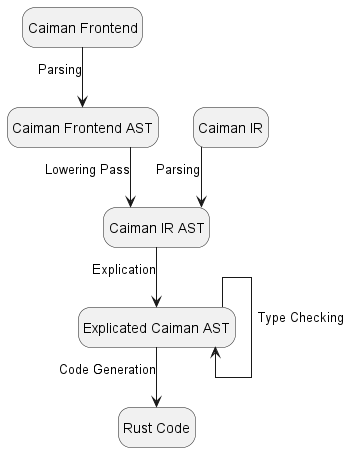
\includegraphics[width=.7\linewidth]{fig/caimanengineering.png}
\label{fig:caiman-compiler}
\caption{Structure of the Caiman Compiler}
\end{figure}

\subsubsection{Caiman to Caiman IR}

Caiman has two distinct representations in the frontend and the IR, resulting in two distinct Abstract Syntax Trees (ASTs).  The transformation from the Caiman frontend AST to the Caiman IR AST is straightforward (if non--trivial to build), needing to transform the specification and implementation logic to the single-operation and SSA style of the Caiman IR.  Specifications (value, timeline, and spatial) in Caiman have no control flow, so translating to the similar representation in Caiman IR requires only (simply) reducing expressions.  

Translating a Caiman implementation to Caiman IR is somewhat more involved, however, as we need to account for the control flow of the function (with respect to the specification) as well as provide information about the allocation of resources in computation.  For conditions, function calls, and recursion, we translated directly for the call site based on the types of the values being used.  We do not currently attempt to implement loops in Caiman.  Allocations are calculated based on value use -- in principle, it would improve explicator flexibility to move allocation logic to the explication search, but we have not practically engineered this approach.

Additionally, both specifications and implementations include standard Hindley-Milner type inference~\cite{Hindley}.  For the implementation language, this type inference is primarily useful for control flow headers (which cannot be explicated), and values not inferred are instead pushed to the explicator for solving.

\subsubsection{Caiman IR explication and typechecking}

To lower the Caiman IR for typechecking, we erase variable and function names and validate program structural assumptions.  We then explicate the program as described in Section~\ref{sec:explication}.  To help make debugging explicated Caiman code manageable, the explicator maintains names throughout, requiring the explicator to retain metadata about the transformed program.  Additionally, at this stage, the explicator performs minimal typechecking to perform explication.  Importantly, however, the explicator makes no guarantee that existing code typechecks, and only intends to produce explicated code that will typecheck if existing code will typecheck.  We do not validate this claim, and instead leave formalizing this connection to future work.

After explication, we guarantee that the explicator either failed to terminate (due to a type error or due to timing out), or every hole in the AST representation of the Caiman IR is filled.  Practically, we represent this state with a duplicate AST with no hole variants.  The typechecker is then able to walk through each function and validate our requirement that each implementation function does the work promised by the implemented specifications, as stated in Section~\ref{sec:formal}.  Additionally, the typechecking pass here validates properties of the allocations and data between funclets, a significant detail of Caiman engineering that is out of scope of this writing.

\subsubsection{Code Generation}
\label{subsec:generation}

Finally, the resulting Caiman IR program is emitted as Rust code, which can then be linked to, compiled, and run.  This Rust code notably includes calls to externally-defined Rust functions and setting up WebGPU API allocations and function calls.  At this stage, code generation makes no attempt to optimize the resulting code (such as inlining code), leaving these additional optimizations to the underlying compiler.

Caiman code generation currently does not support directly emitting WebGPU code, and as a result treats each WebGPU function as a black--box call.  It is possible to fuse these calls, or even to emit WebGPU directly in Caiman, but these additions are not yet implemented.  This detail can lead to significant performance loss, and certainly would require an implementation to use Caiman in a practical setting.

\section{Results}
\label{sec:results}

At the time of this writing, quantitative results of Caiman are minimal and not worth reporting.  We have, however, implemented around 100 synthetic examples of Caiman programs, which can give qualitative insight into the current implementation of Caiman described.  Intended future performance measurements will be summarized in Section~\ref{subsec:future}.

The programs implemented in Caiman are intended primarily for testing, but provide some idea of the flexibility of our produced implementation.  Notable examples of Caiman programs include the following, the full code of which is included in Appendix~\ref{subsec:caiman-frontend-examples}:

\begin{itemize}
\item Nested conditional logic
\item Recursive functions 
\item WebGPU function calls, including conditional logic and recursive calls
\item Fixed-sized arrays
\item \code{select_sum}, as described in Section~\ref{sec:practical}
\end{itemize}

In developing these examples, we have found that Caiman's type system is remarkably flexible, though it takes time to become comfortable with implementing Caiman code.  Specifically, implementing a Caiman specification requires some amount of care when breaking up the specification and managing types of each operation in cases where type inference is insufficient.  

This being said, the Caiman type system has caught dozens of errors we have made while implementing these functions, including mistakes in managing control flow when calling into the GPU.  We have also found that, practically, Caiman programs can be written essentially as we might expect despite the specificity of Caiman's type requirements.  

The main issue we have had implementing programs is that some implementation rewrites are restricted under Caiman's type system without changing the specification, which is precisely what we would like to avoid.  A notable example of this weakness is the technical detail described in Section~\ref{subsec:generation}, where the Caiman semantics is insufficient for merging two calls that we know to be equivalent to a specific single function call.

We have not yet implemented functions that significantly and scientifically test Caiman's resulting runtime performance.  Qualitatively, all Caiman programs we have written run nearly instantly, but without comparison to directly written WebGPU programs, this result is, bluntly, insufficient to draw any real conclusions.

\subsection{Explication}
\label{subsec:explicationresults}

Explication is the most likely stage of Caiman compilation to produce interesting timing results, both in terms of the time of compilation and the runtime of these programs.  We have implemented synthetic examples of explication, with at most 30 lines of code for a given explication implementation.  Notably, however, at the time of this writing, we have not fully implemented the \code{???} statement described in Section~\ref{sec:explication}.

At the time of this writing, qualitatively, the explication examples we have written compile and run nearly instantly.  We expect this to be similarly instant for an implementation written entirely with a \code{???} statement.  Where we expect to see the pathologically slow examples are in functions that use a mix of \code{???} statements and a small number of restricted expressions, where the greedy search done by the explicator becomes less likely to quickly find a solution.  We expect these cases to scale exponentially with the number of lines in a given funclet.

\section{Conclusion}
\label{sec:conclusion}

We have argued that writing performant heterogeneous operations often requires experimentation with multiple function implementations of the same underlying operation.  We have seen how this gap between intent and implementation can lead to programmer mistakes and maintaining a combinatorial explosion of function implementations.

With Caiman, we have shown a mechanism by which we can separate the specification and implementation of such heterogeneous operations.  We have shown how we can represent control flow and recursive operations in a specification and how to verify that an implementation associated with a specification will calculate the data as we expect.

We have also examined how we can use explication to automate generation of these implementations, and specifically in such a way that this automation can be broken down.  More concretely, we have examined how automating the generation of programs can be controlled through providing both a specification and precise line--by--line generation requirements.

Finally, we have described our specific implementation for CPU/GPU code to generate Rust code to interface with WGPU.  We have also shown the structure of the Caiman compiler, and have hinted how code generation can be replaced to work in a variety of heterogeneous settings.

\subsection{Future Work}
\label{subsec:future}

Most immediately, timing information about explication and generated Caiman code will be gathered and reported.  Such data will allow for more concrete and narrow arguments as to the efficacy of our Caiman implementation and an examination of the potential scalability of explication.

An important observation about the explication results we have observed is that the explicator does not attempt to reason about the interactions between multiple funclets.  Introducing general control flow to the explicator would \emph{likely} reduce performance (and expand engineering needs) substantially.  This being said, implementing explication in such a way as to generate functions to fill in control flow seems relatively achievable, and would help substantially in implementation details that currently need to be written by hand.

The remainder of this section will discuss potential directions for Caiman that have been discussed, but not implemented.

Caiman's implementation in Rust with WebGPU is fairly narrow and can be difficult to manage.  Implementing Caiman to directly generate code for an IR (such as Cranelift~\cite{cranelift} or LLVM~\cite{llvm}) would improve Caiman's usability and transparency tremendously.  Additionally, targeting Vulkan would make more practical sense in exposing more details in the Caiman communication model.

It would be very interesting to explore an implementation of Caiman targeting either compute (with CUDA or OpenCL), or another device entirely.  Caiman seems directly useful for multiple--device code architectures, or for using another non--CPU host (such as GPU--driven logic).  Caiman was also designed with FPGAs and network chips in mind, though without an implementation, how effective this design transfers is completely untested.

Rewriting kernels entirely in Caiman seems impractical in many cases, but it also seems conceptually straightforward to write a translator from a subset of C or CUDA to a Caiman specification.  Such tooling could have clear practical advantages, allowing a user to harness the type--level power of Caiman without needing to rewrite every specification by hand.  The untested downside of this approach could be that Caiman's type system would be too rigid to allow such a straightforward translation, and this would require practical experimentation.

Finally, Caiman explication code can be difficult to debug, particularly in cases where the explicator is directed incorrectly and generates a bunch of strangely--named nonsense that exposes some mistake in the specification.  The explication step we have described and implemented is transparent to the compiler, however, and there is an interesting potential HCI challenge in exploring an approach to improve Caiman error messages or provide some sort of visual or IDE tooling to examine explicated Caiman code.